\documentclass[12]{beamer}
\usepackage[utf8]{inputenc}
%\usepackage[T1]{fontenc}
\usepackage{lmodern}
\usepackage{hyphsubst}%
\usepackage{semtrans}
\usepackage{amsthm}
\usepackage{amsfonts}
\HyphSubstIfExists{ngerman-x-latest}{%
  \HyphSubstLet{ngerman}{ngerman-x-latest}}{}
\HyphSubstIfExists{german-x-latest}{%
  \HyphSubstLet{german}{german-x-latest}}{}
%\usepackage[english,ngerman]{babel}
\usepackage{textcomp}
\usepackage{microtype}
\beamerdefaultoverlayspecification{<+->}

\usetheme{Luebeck}
% Copenhagen
% Dresden
% Hannover
% Luebeck
% Montpellier
% Pittsburgh
% Singapore

\title{Text Generation with LSTM Units}
% \author{Antonio Bozzano Schwedhelm}
\author{By Me}
\date{\today}

\begin{document}
\begin{frame}
\titlepage
\end{frame}
%presentation is about a project i did a couple of months ago

\section{Introduction}
\begin{frame}
\frametitle{Introduction}
\begin{itemize}
\item<1-> I wanted to replicate the results shown in the blog post ``The Unreasonable Effectiveness of Recurrent Neural Networks''.
\item<2-> I also wanted to have fun.
\end{itemize}
\end{frame}
%really recomend this
%exciting time to be alive

%used favourite language: c++
%did it from scratch and made my own matrix class

\section{How Neural Networks Work}
\begin{frame}
\frametitle{How Neural Networks Work}
\begin{itemize}
\item<1-> In general:
$$f_w:\left(-1,1\right)^n\longmapsto\left(-1,1\right)^m$$
\item<2-> Or:
$$f_w:\left(0,1\right)^n\longmapsto\left(0,1\right)^m$$
\end{itemize}
\end{frame}
%or a combination

\begin{frame}
\frametitle{How Neural Networks Work}
\begin{itemize}
\item<1-> A neural network consists of layers.
\item<1-> The first layer receives the input, transforms it, and passes it on to the next layer.
\item<1-> Each subsequent layer receives an array from the previous layer, transforms it, and passes it on.
\item<1-> The output of the last layer is the output of the neural network.
\item<2-> Transformation: Multiply the input with a matrix and apply a function to each element of the result.
\end{itemize}
\end{frame}

\begin{frame}
\frametitle{How Neural Networks Work}
\begin{center}
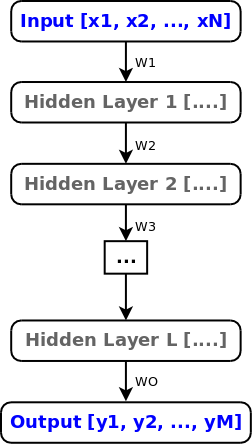
\includegraphics[scale=0.25]{../images/network01.png}
\end{center}
\end{frame}
%do not make a "neuron" class or anythin similar
%you could look at each neuron and each weight individually. In general, this is a bad idea

\begin{frame}
\frametitle{How Recurrent Neural Networks Work}
\begin{center}
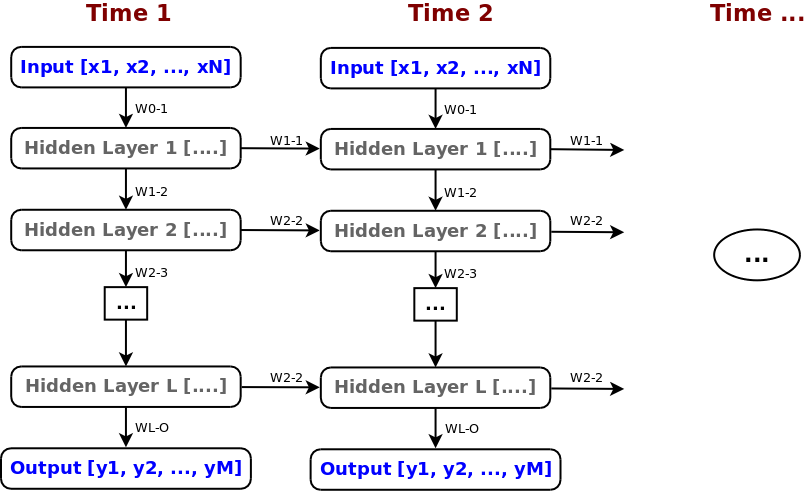
\includegraphics[scale=0.25]{../images/network02.png}
\end{center}
\end{frame}
%and of course, you can do whatever you want here
%layers may or may not be connected in time

\section{My Project}
\begin{frame}
\frametitle{The Input}
\end{frame}

\begin{frame}
\frametitle{The output}
\end{frame}

\begin{frame}
\frametitle{What Kinds of Layers are Needed}
\begin{itemize}
\item<1-> I needed three kinds of layers:
\begin{itemize}
\item<1-> Tanh Layers.
\item<1-> LSTM Layers.
\item<1-> Softmax Layers.
\end{itemize}
\end{itemize}
\end{frame}

\begin{frame}
\frametitle{How Does a Tanh Layer Work}
\begin{itemize}
\item<1-> It is a simple mapping: $f_w:\left(-1,1\right)^n\longmapsto\left(-1,1\right)^m$.
\end{itemize}
\end{frame}
%in my case, input can also be (0,1)

\begin{frame}
\frametitle{How Does a LSTM Layer Work}
\begin{itemize}
\item<1-> It is also a mapping: $f_{w,s}:\left(-1,1\right)^n\longmapsto\left(-1,1\right)^m$.
\item<1-> But it has an internal state, meaning that previous runs of the neural network may influence the output.
\end{itemize}
\end{frame}

\begin{frame}
\frametitle{How Does a Softmax Layer Work}
\begin{itemize}
\item<1-> It is a mapping: $f_w:\left(-1,1\right)^n\longmapsto\left(0,1\right)^m$.
\item<1-> Where the output values add up to one, so that the output can be interpreted as a probability distribution.
\end{itemize}
\end{frame}
%again, this is in my case, input can also be (0,1)

\section{End}
\begin{frame}
\frametitle{The end}
\end{frame}

\end{document}